\section{PSICOV}

    \subsection{Gaussian graphical models} 

        PSICOV relies on a Gaussian graphical modelization. Such models are represented by undirected graphs that
        satisfy the pairwise Markov property: two nodes are not connected by an edge if they are conditionally independent.
        Let $G = (V, E)$ be a graph and let each node $k$ be associated to a random variable $X_k$.
        Conditional independence between variables $X_u$ and $X_v$ is formally defined as follows:
        \begin{equation}
            X_u \independent X_v \vert X_{V \\ \{u, v\}} \, \, \text{if } \{u, v\} \notin E
        \end{equation}
        If the graph is not complete, then there exists pairs of conditionally independent variables in the model,
        resulting in sparsity patterns in the underlying precision matrix.
        When the covariance matrix of the multivariate Gaussian model is rank-deficient, a solution for the precision
        matrix has to be found with a high prior towards sparse matrices. Such a solution can be achieved through
        regularization. The solution that follows in the next section relies on pseudo-inverse computation
        with L1 regularization.

    \subsection{Evolutionary couplings} \label{graphicalmodels}

        The motivation behind PSICOV~\cite{doi:10.1093/bioinformatics/btr638} is that residue contacts produce constraints on the types of residues in the
        protein at certain pairs of sites: two residues involved in a contact should have complementary physicochemical properties. To capture the covariation
        of residue types for any pair of sites, the random variable $X_{ia}: \Omega \rightarrow \{0, 1\}$ is defined. $X_{ia}$ takes value one if
        amino acid at site $i$ is of type $a$. In particular, value $x_{ia}^{(k)}$ is equal to one if the $k$th sequence in the given MSA has a residue of type $a$
        at site $i$. tWith this knowledge, the sample covariance matrix $S \in \mathbb{R}^{21 L \times 21 L}$ can then be computed by:

        \begin{equation} \label{covariance}
            \begin{split}
                S_{ij}^{ab} & = \frac{1}{n} \sum\limits_{k=1}^{n} \big( x_{ia}^{(k)} - \bar{x}_{ia} \big) \big( x_{jb}^{(k)} - \bar{x}_{bj} \big)
            \end{split}
        \end{equation}

        where s$n$ is the number of
        homologuous sequences and $S_{ij}^{ab}$ is the sequence identity covariance from amino acid $a$ to amino acid $b$ and from site $i$ to site $j$.
        Each matrix $S_{ab}$ is thus a covariance matrix between sites $i$ and $j$. It is noteworthy that such a covariance matrix is neither positive
        semidefinite nor symmetric and is, thus, substantially different from regular sample covariance matrices. Precision matrix $\Theta_{ij}$ is defined as
        the inverse of covariance submatrix $S_{ij}$, but there is no guarantee that such an inverse can be computed directly. Indeed, each submatrix
        $S_{ij}$ is very likely to be singular due to the absence of correlations for some residue types that are rarely (or never) observed at given sites.

        \begin{figure}[H]
            \begin{center}
                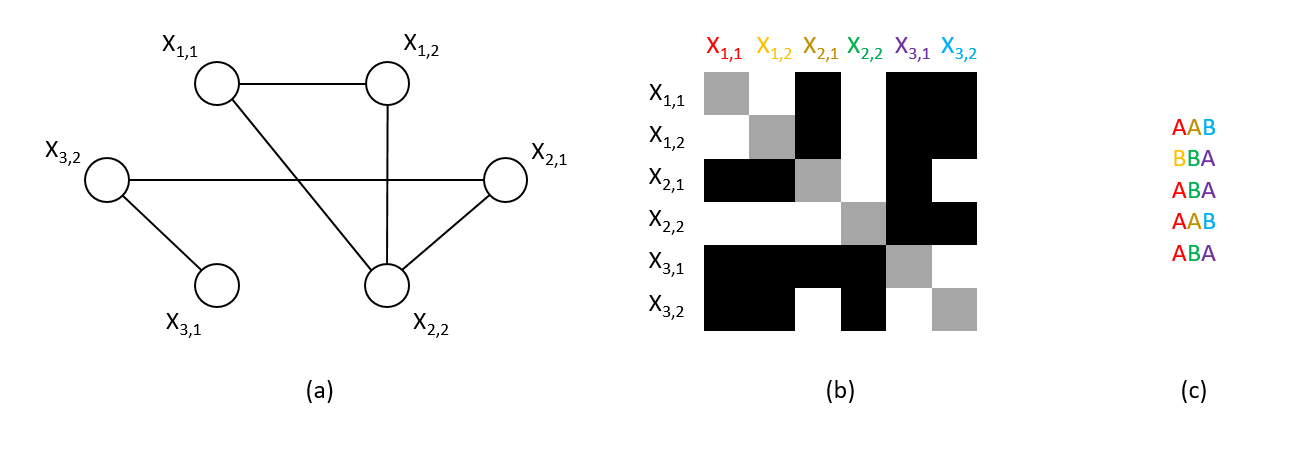
\includegraphics[width=\textwidth, keepaspectratio]{imgs/ggm.png}
                \caption{Illustration of a small system with only 3 sites and 2 amino acid types A and B:
                    (a) Gaussian graphical model representing the system.
                    (b) Sparsity pattern of the estimated inverse covariance matrix.
                    Cells associated to zero variables are drawn in black. (c) Corresponding MSA.}
                \label{thresholds}
            \end{center}
        \end{figure}

    \subsection{Inference}

        The solution chosen here is to estimate sparse inverse covariance matrices instead,
        by having recourse to Graphical Lasso algorithm~\cite{graphicalLasso}.
        The method assumes that observations follow a multivariate normal distribution
        characterized by the following probability density function:

        \begin{equation}
            f(x) = \frac{1}{\sqrt{(2\pi)^k \vert\Sigma\vert}} \exp{-\frac{1}{2} (x - \mu)^T \Sigma^{-1} (x - \mu)}
        \end{equation}

        where $d=21L$ is the number of components in vector $x$, $\mu$ is the theoretical mean and $\Sigma$ the theoretical covariance matrix.
        Let's express the log-likelihood of the data as a function of the inverse theoretical matrix $\Theta$:

        \begin{equation}
            \begin{split}
                \log{L}(\Theta) & = \sum\limits_{k=1}^{n} \log{f(x^{(k)})} \\
                & = \sum\limits_{k=1}^{n} \Bigg( -\frac{1}{2} (x^{(k)} - \mu)^T \Sigma^{-1} (x^{(k)} - \mu) - \log{\sqrt{(2\pi)^d \vert\Sigma\vert}} \Bigg) \\
                & = \sum\limits_{k=1}^{n} \Bigg( -\frac{1}{2} (x^{(k)} - \mu)^T \Theta (x^{(k)} - \mu) - \log{\sqrt{(2\pi)^d \frac{1}{\vert\Theta\vert}}} \Bigg) \\
                & = -\frac{1}{2} \sum\limits_{k=1}^{n} (x^{(k)} - \mu)^T \Theta (x^{(k)} - \mu) 
                    - \frac{1}{2} \sum\limits_{k=1}^{n} \log{\Big((2\pi)^d \frac{1}{\vert\Theta\vert}\Big)} \\
                & = -\frac{1}{2} \trace\big(S \Theta\big) - \frac{1}{2} \sum\limits_{k=1}^{n} \log{(2\pi)^d} + \frac{1}{2} \log{\vert\Theta\vert} \\
            \end{split}
        \end{equation}

        The latter expression holds because the empirical mean $\bar{x}$ is equal to $\mu$ for any $\Sigma$.
        The objective function of Graphical Lasso is simply the log-likelihood penalized with $L_1$ norm. $L_1$ regularization is used instead of $L_2$ because
        of its non-asymptotic behaviour and therefore its ability to produce more zeroes among the parameter values.
        The solution to the optimization problem is described as:

        \begin{equation}
            \begin{split}
                \hat{\Theta} & = \argmax_{\Theta} \ \ \log{L}(\Theta) - \rho \norm{\Theta}_1 \\
                & = \argmax_{\Theta} \ \ -\frac{1}{2} \trace\big(S \Theta\big) - \frac{1}{2} \sum\limits_{k=1}^{n} 
                    \log{(2\pi)^d} + \frac{1}{2} \log{\vert\Theta\vert} - \rho \norm{\Theta}_1 \\
                & = \argmax_{\Theta} \ \ -\trace\big(S \Theta\big) + \log{\vert\Theta\vert} - \rho \norm{\Theta}_1 \\
            \end{split}
        \end{equation}

        The $L_1$ norm $\norm{\Theta}_1$ is the sum of absolute values of the elements in $\Theta$.
        \todo{}

        \todo{Optimizer, GLassoFast, etc.}

        \todo{APC}

        According to Sun et al.~\cite{doi:10.1093/nar/gky995}, the solutions found by PSICOV may not be suitable for some proteins.
        Furthermore, the best solution could be far from the global optimum found by Graphical Lasso since the search space is huge.
        The suggested solution is to predict multiple contact maps and promote diversity among them by adding a new penalty term.

        \begin{equation}\label{mbest}
            \begin{split}
                & min_{\Theta^{(m+1)}} \frac{1}{2} \trace\big(S \Theta\big) + \frac{1}{2} 
                    \sum\limits_{k=1}^{n} \log{(2\pi)^d} - \frac{1}{2} \log{\vert\Theta\vert} \\
                & s.t. \ \ \ d(\Theta^{(k)}, \Theta^{(m+1)}) \ge \epsilon, \ \ k = 1, \dotsc, m
            \end{split}
        \end{equation}

        In that last equation, the distance constraint function $d$ is a convex and differentiable function defined as:

        \begin{equation}
            d(\Theta^{(k)}, \Theta) = - \sum\limits_{i, j} \delta_0(\theta^{(k)})_{i, j} \vert \Theta_{i, j} \vert
        \end{equation}

        where $\delta_0: \mathbb{R}^{21L \times 21L} \rightarrow \mathbb{R}^{L \times L}$ is such that 
        $d(\Theta_{i, j})$ takes value $1$ if submatrix $\Theta_{i, j}$ is $0$, and $-1$ otherwise.
        The objective function is optimized using a second-order method and updating the solution in the Newton direction at each iteration.
        Finally, a contact map is obtained by selecting the submatrices among the solutions according to their sparsity.
        More specifically, submatrices are selected according to their nuclear norm, hence the sum of their singular values.
